\documentclass[11pt, unicode, aspectratio=169]{beamer}

\usepackage{luatexja}

\usetheme{Madrid}
\usecolortheme{default}
\usefonttheme{serif}
\setbeamertemplate{navigation symbols}{}

\usepackage{amsmath, amssymb, amsthm, mathtools}
\usepackage{bm}
\usepackage{physics}
\usepackage{graphicx}
\usepackage{tikz}

\title{一端を固定された紐の落下挙動の解析}
\author{黒瀬 諭一朗}
\institute{埼玉県立大宮高等学校物理部}
\date{\today}

\begin{document}

\begin{frame}
  \titlepage
\end{frame}

\begin{frame}{研究の背景と目的}
  \textbf{背景}
  \begin{itemize}
    \item 先行研究の32重振り子の落下シミュレーションにおける観察．
    \item 振り子が\textbf{初期状態の直線を保ったまま落下}しようとする．
    \item 時間経過とともに\textbf{固定端側から折れ曲がっていく}現象．
  \end{itemize}
  \vspace{1em}
  
  \textbf{疑問と目的}
  \begin{itemize}
    \item 「紐という連続的な物体はどのように運動するのか？」
    \item \textbf{一端を固定された紐の自由落下挙動を数学的に解明する}．
  \end{itemize}
\end{frame}

\begin{frame}{解析手法：定式化}
  \begin{columns}
    \begin{column}{0.6\textwidth}
      \textbf{仮定とモデル}
      \begin{itemize}
        \item 紐は\textbf{太さと曲げ剛性を持たない}．
        \item 長さ $l$ ，質量 $m$ の紐を $N$ 等分する．
        \item 長さ $\Delta l = l / N$ の剛体棒と質量 $\Delta m = m / N$ の質点からなる\textbf{$N$重振り子}として定式化．
        \item 初期状態：鉛直線と角度 $\theta$ をなす直線上で静止．
      \end{itemize}
    \end{column}
    \begin{column}{0.4\textwidth}
      \centering
      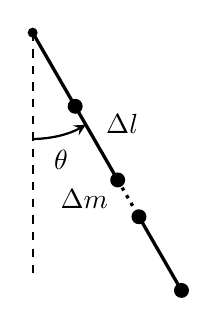
\begin{tikzpicture}[scale=0.9, >=stealth]
        % 固定端（原点）
        \coordinate (O) at (0,0);
        \fill (O) circle (2.0pt);
        % 鉛直線
        \draw[dashed, thick] (O) -- (0, -3.5);
        % 角度
        \draw[->, thick] (0, -1.5) arc[start angle=-90, end angle=-60, radius=1.5];
        \node at (0.4, -1.8) {$\theta$};
        % 振り子
        \def\ang{-60}
        \coordinate (P1) at (\ang:1.2);
        \coordinate (P2) at (\ang:2.4);
        \coordinate (P3) at (\ang:3.0);
        \coordinate (P4) at (\ang:4.2);
        \draw[very thick] (O) -- (P1);
        \draw[very thick] (P1) -- (P2);
        \draw[very thick, dotted] (P2) -- (P3);
        \draw[very thick] (P3) -- (P4);
        % 質点
        \fill (P1) circle (3pt);
        \fill (P2) circle (3pt) node[below left] {$\Delta m$};
        \fill (P3) circle (3pt);
        \fill (P4) circle (3pt);
        \node at (\ang:1.8) [above right] {$\Delta l$};
      \end{tikzpicture}
    \end{column}
  \end{columns}
\end{frame}

\begin{frame}{解析手法：アプローチ}
  \textbf{微小時間の仮定とテイラー展開}
  \begin{itemize}
    \item 落下挙動を調べるため，時刻 $t$ は微少量であると仮定．
    \item 時刻 $t=0$ における各質点の角加速度を $\alpha_k$ とおく．
    \item 角度 $\varphi_k$ をテイラー展開で近似：
      \begin{equation}
        \varphi_k = \theta + \frac{1}{2} \alpha_k t^2
      \end{equation}
  \end{itemize}
  \vspace{1em}
  
  \textbf{解析の流れ}
  \begin{enumerate}
    \item 運動エネルギーとポテンシャルからラグランジアン $L$ を構成．
    \item ラグランジュ方程式から初角加速度 $\alpha_j$ に関する連立方程式を導出．
    \item \textbf{$N \rightarrow \infty$ の極限}を取り，連続体としての挙動を解析．
  \end{enumerate}
\end{frame}

\begin{frame}{結果：ラグランジアンの構成（座標と変数の設定）}
  \textbf{座標と変数の設定}
  \begin{itemize}
    \item 固定端を原点とし，地面と平行に$x$軸，鉛直下向きに$y$軸を取る．
    \item 自由落下開始時刻を，$t = 0$とする．
    \item 時刻$t$における$j$番目の質点が鉛直線となす角度を$\varphi_j$とする．
    \item 時刻$t$における$i$番目の質点の座標$\left(x_i, y_i\right)$は次のように表される：
      \begin{equation}
        x_i = \Delta l \sum_{j = 1}^{i} \sin \varphi_j, \quad y_i = \Delta l \sum_{j = 1}^{i} \cos \varphi_j
      \end{equation}
    \item 時刻$t$における$i$番目の質点の速度$\left(\dot{x_i}, \dot{y_i}\right)$は次のように表される：
      \begin{equation}
        \dot{x_i} = \Delta l \sum_{j = 1}^{i} \dot{\varphi_j} \cos \varphi_j,\quad \dot{y_i} = \Delta l \sum_{j = 1}^{i} \dot{\varphi_j} \sin \varphi_j
      \end{equation}
  \end{itemize}
\end{frame}

\begin{frame}{結果：ラグランジアンの構成（運動エネルギーの導出）}
  系の運動エネルギー$T$：
  \begin{equation}
    T = \frac{1}{2} \Delta m \sum_{i = 1}^{N} \left(\dot{x_i}^2 + \dot{y_i}^2\right)
  \end{equation}
  (3)を代入して整理すると：
  \begin{equation}
    T = \frac{1}{2} \Delta m {\Delta l}^2
      \sum_{i = 1}^{N} \sum_{j = 1}^{i} \sum_{k = 1}^{i}
      \dot{\varphi_j} \dot{\varphi_k} \cos \left(\varphi_j - \varphi_k\right)
  \end{equation}
  和の順序を入れ替えると：
  \begin{equation}
    T = \frac{1}{2} \Delta m {\Delta l}^2
        \sum_{j = 1}^{N} \sum_{k = 1}^{N} \left(N - \max \left(j, k\right) + 1\right)
        \dot{\varphi_j} \dot{\varphi_k} \cos \left(\varphi_j - \varphi_k\right)
  \end{equation}
\end{frame}

\begin{frame}{結果：ラグランジアンの構成（ポテンシャル・エネルギーの導出）}
  系のポテンシャル・エネルギー$U$：
  \begin{equation}
    U = - \Delta m g \sum_{i = 1}^{N} y_i
  \end{equation}
  (2)を代入すると：
  \begin{equation}
    U = - \Delta m g \Delta l \sum_{i = 1}^{N} \sum_{j = 1}^{i} \cos \varphi_j
  \end{equation}
  和の順序を入れ替えると：
  \begin{equation}
    U = - \Delta m g \Delta l \sum_{j = 1}^{N} \left(N - j + 1\right) \cos \varphi_j
  \end{equation}
\end{frame}

\begin{frame}{結果：ラグランジアンの構成}
  (6)，(9)より，ラグランジアン$L = T - U$が構成される：
  \begin{equation}
    \begin{aligned}
      L &= \frac{1}{2} \Delta m {\Delta l}^2
           \sum_{j = 1}^{N} \sum_{k = 1}^{N} \left(N - \max \left(j, k\right) + 1\right)
           \dot{\varphi_j} \dot{\varphi_k} \cos \left(\varphi_j - \varphi_k\right) \\
        & \quad + \Delta m g \Delta l \sum_{j = 1}^{N} \left(N - j + 1\right) \cos \varphi_j
    \end{aligned}
  \end{equation}
\end{frame}

\begin{frame}{結果：$N \rightarrow \infty$ の極限と積分方程式}
  ラグランジュ方程式から得られた連立方程式に対し，固定端からの長さを $s' = j \Delta l$ , $s = k \Delta l$ と対応させて $N \rightarrow \infty$ の極限を取る．
  
  \vspace{1em}
  和が積分に置き換わり，初角加速度 $\alpha(s')$ に関する以下の\textbf{積分方程式}を得た：
  \begin{equation*}
    \int_{0}^{l} \left(l - \max(s', s)\right) \alpha(s') \,ds' + g(l - s)\sin\theta = 0
  \end{equation*}
  \vspace{1em}
  両辺を $s$ について微分して整理すると：
  \begin{equation*}
    \int_{0}^{s} \alpha(s') \,ds' = -g \sin\theta
  \end{equation*}
\end{frame}

\begin{frame}{結果：解の導出とデルタ関数の出現}
  得られた積分方程式：
  $$ \int_{0}^{s} \alpha(s') \,ds' = -g \sin\theta $$
  
  \vspace{1em}
  $s > 0$ において両辺を微分すると $\alpha(s) = 0$ となる．
  この条件を満たすためには，解に\textbf{ディラックのデルタ関数} $\delta(s)$ が必要となる．

  \vspace{1em}
  \textbf{最終的な初角加速度と角度：}
  \begin{align*}
    \alpha(s) &= -g \sin\theta \cdot \delta(s) \\
    \varphi(s) &= \theta - \frac{1}{2}gt^2 \sin\theta \cdot \delta(s)
  \end{align*}
\end{frame}

\begin{frame}{考察}
  \textbf{自由端側の平行移動}
  \begin{itemize}
    \item $s > 0$ において $\varphi(s) = \theta$ 
    \item 自由端側の紐は，剛体棒のように\textbf{初期状態の直線を保ったまま平行移動的に落下}しようとする．
  \end{itemize}
  \vspace{1em}

  \textbf{固定端における特異点}
  \begin{itemize}
    \item $s = 0$ において角度 $\varphi(s)$ が無限大になる．
    \item 原因：「紐全体を直線に保とうとする慣性」と「固定端の拘束力」の衝突．
  \end{itemize}
\end{frame}

\begin{frame}{結論と今後の展望}
  \textbf{結論}
  \begin{itemize}
    \item 紐は自由落下を開始した直後，固定端以外の部分は直線を保ったまま落下しようとする．
    \item しかし固定端にはデルタ関数的な特異性が現れ，数学的結果と物理的現実との間に矛盾が生じた（現実には角度が無限大になることはない）．
  \end{itemize}
  \vspace{1em}

  \textbf{今後の展望}
  \begin{itemize}
    \item 現実の紐が持つ「太さ」や「曲げ剛性」を考慮に入れる．
    \item $t$ の3次以上の項を無視した微小時間だけでなく，\textbf{有限な時間経過における落下挙動}（折れ曲がりの伝搬など）を解析する手法の構築．
  \end{itemize}
\end{frame}

\end{document}
